\section{Speed and Memory Footprint}
Implementing the technique of the previous section may be considered too costly.
First, it inserts many instructions before realizing most are useless, and copy
insertion is already by itself time-consuming. 
It introduces many new variables, too.
The size of the variable universe has an impact on the liveness analysis and
the interference graph construction. Also, if a general coalescing algorithm is used, a
graph representation with adjacency lists (in addition to the bit matrix) and a
working graph to explicitly merge nodes when coalescing variables, would be
required.  All these constructions, updates, manipulations are 
time-consuming and memory-consuming.  We may improve the whole process
by: a) avoiding the use of any interference graph and liveness sets; b) avoid the quadratic complexity of interference check between two sets of variables by an optimistic approach that first coalesces even interfering variables, then traverses each set of coalesced variables and un-coalesce one by one all the interfering ones\ifhab(this is the technique advocated by Budimlic et al. in~\cite{liverange.pldi02})\fi; c) emulating (``virtualizing'') the introduction of the
$\phi$-related copies.

\paragraph{Interference check}
Liveness sets and interference graph are the major source of memory usage. This motivates, in the context of JIT compilation, not to build any interference graph at all, and rely on the liveness check described in Chapter~\ref{chapter:liveness} to test if two live-ranges intersect or not. Let us suppose for this purpose that a ``has-the-same-value'' equivalence relation, is available thanks to a mapping $V$ of variables to symbolic values: \\
$$\textrm{variables }a\textrm{ and }b\textrm{ have the same value } \Leftrightarrow V(a)=V(b)$$
As explained in Paragraph~\ref{par:alternative_ssa_destruction:value} this can be done linearly (without requiring any hash map-table) on a single traversal of the program if under strict SSA form. 
We also suppose that liveness check is available, meaning that for a given variable $a$ and program point $p$, one can answer if $a$ is live at this point through the boolean value of  $a.\textit{islive}(p)$. This can directly be used, under strict SSA form, to check is two variables live-ranges, say $a$ and $b$ intersect:
$$\begin{array}{rcl}
\intersect(a,b) & \Leftrightarrow & \textit{liverange}(a)\cap \textit{liverange}(b)\neq\emptyset\\
 & \Leftrightarrow & \left\lwave
\begin{array}{l}
\textit{a.def.op}=\textit{b.def.op}\\
\textit{a.def.op} \textrm{ dominates } \textit{b.def.op} \bigwedge \textit{a.islive}\left(\textit{out}(\textit{b.def.op})\right)\\
\textit{b.def.op} \textrm{ dominates } \textit{a.def.op} \bigwedge \textit{b.islive}\left(\textit{out}(\textit{a.def.op})\right)\\
\end{array}\right.
\end{array}
$$

Which leads to our refined notion of interference:

$$\interfere(a,b) \Leftrightarrow \intersect(a,b) \bigwedge V(a)\neq V(b)$$

\paragraph{De-coalescing in linear time}
The interference checking outlined in the previous paragraph allows to avoid building an interference graph of the SSA form program. However, coalescing has the effect of merging vertices and interference queries are actually to be done between sets of vertices. Using an interference graph, one can manipulate a \emph{working graph} which vertices corresponds to sets of coalesced variables, and update it along ongoing coalescing. Without any interference graph, one can ``naively'' test a quadratic number of interferences for each interference query. With more efforts\ifhab~\cite{Boissinot09}\fi, linear complexity is possible, but the technique considered here is even more radical. The idea is to first merge all copy and \phifun related variables together. A merged-set might of course contain interfering variables at this point. The idea is to identify some variables that interfere with some other variables within the merged-set, and remove them from the merged-set. As we will see here, thanks to the dominance property, this can be done linearly using a single traversal of the set.

In reference with register allocation, and graph coloring, we will associate the notion of colors to merged-sets: every variables of the same set are assigned the same color, and different sets are assigned different colors. The process of \emph{de-coalescing} a variable is to extract it from its set; it is not put in another set, just isolated. So we will refer such a variable as \emph{un-colored}. Actually, variables pined together have to stay together. So the process of un-coloring a variable might have the effect of un-coloring some others. In other words, a colored variable is to be coalesced with variables of the same color, and any un-colored variable is to be coalesced only with the variables it is pined with. 


We suppose that variables have already been colored and the goal is to un-color some of them (preferably not all of them) so that each merged-set become interference free. We suppose that if two variables are pined together they have been assigned the same color, and that a merged-set cannot contain variables pined to different physical resources. Here we focus on a single merged-set and the goal is to make it interference free within a single traversal. The idea\ifhab advocated by Budimlic et al.~\cite{Budimlic02} \fi exploits the tree shape of variables live-ranges under strict SSA. To this end, variables are identified by their definition point and ordered using dominance accordingly. Traversal of the set is performed along the dominance order, enforcing at each step the sub-set of already considered variables to be interference free. From now, we will abusively design as the dominators of a variable $v$, the set of variables of \emph{identical color than $v$} which definition dominate the definition of $v$. Variables defined at the same program point are arbitrarily ordered, so as to use the standard definition of immediate dominator (denoted $\cidom{v}$, set to $\undef$ if not exists).

First, consider the example of Figure~\ref{fig:alternative_ssa_destruction:fig:domtree} to illustrate the following properties. Consider the current variable $v$,  and an interfering dominating variable $\curanc$. Clearly, \curanc\ intersects (or is identical to) $\cidom{v}$: for our example, as $a$ does not intersect $\cidom{c}=b$ it cannot intersect $c$. On the other-end, with $e$ as the current variable, the intersection of $e$ with $a$ implies the intersection of $a$ with $\cidom{e}=d$. If by construction $d$ and $a$ do not interfere this implies that $V(a)=V(d)$... 
%
As a consequence, if one suppose that at a given step the set of dominating variables is interference free, checking if the current variable, say $v$, interferes with one of its dominating ones, consists in: (1) check if $v$ interfere with its immediate dominator, $u=\cidom{v}$; (2) if not, walk-up the dominators ($\curanc$) of $u$ that both intersect $u$ and have the same value $V$ than $u$: check the interference with $v$. Walking up along this set is done in Algorithm~\ref{alg:alternative_ssa_destruction:domup}, through the use of $\eanc{v}$ that points to the immediate dominating such variable. In this algorithm, we suppose that traversing the merged-set along the dominance order is possible, and that dominance test is available. As for the standard renaming pass during SSA construction, the $\textit{idom}$ field is set during the traversal as the updated value of \curidom.  


\begin{figure}
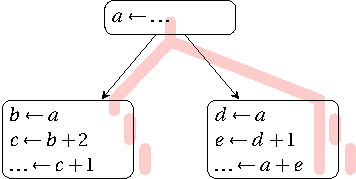
\includegraphics[width=0.6\textwidth]{domtree.pdf}
\caption{\label{fig:alternative_ssa_destruction:fig:domtree}Variables live-ranges are sub-trees of the dominator tree}
\end{figure}

\begin{algorithm}[h]
$\curidom=\undef$\;
\ForEach{variable $v$ of the merged-set in DFS pre-order of the dominance tree}{
  \tcc{Finds and set the immediate dominator of $v$}
  $u \gets \curidom$\;
  \While{$(u \neq \undef) \bigwedge \left(\neg(u \dominates\ v) \vee \uncolored(u)\right)$}{
         $u \gets \cidom{u}$\;
  }
  $\cidom{v}\gets u$\;
  $\curidom \gets v$\;
  \tcc{Walk up variables that have the same value than $u$\\
    Do it until $v$ is uncolored or no more interference with $v$} 
  $\eanc{v}\gets \undef$\;
  $\curanc \gets u$\;
  \While{$\curanc\neq\undef$}{
    \tcc{Find the first one that intersects $v$ with the same color than $u$}
    \While{$\curanc\neq \undef \bigwedge 
      \neg\left(\colored(\curanc) \wedge \intersect(\curanc,v)\right)$}{
      $\curanc \gets \eanc{\curanc}$\;
    }
    \If{$\curanc \neq \undef$}{
      \If{$V(\curanc) = V(v)$}{
	$\eanc{v} \gets \curanc$\;
	break \;
      }
      \Else { \tcc{$\curanc$ and $v$ interfere}
        \If{preferable to uncolor $v$}{
          uncolor $v$\;
          break\;
        } 
        \Else {
          uncolor $\curanc$\;
          $\curanc \gets \eanc{\curanc}$\;
        }
      }
    }
  }
}
\caption{\label{alg:alternative_ssa_destruction:domup} De-coalescing of a merged-set}
\end{algorithm}

\paragraph{Virtualizing $\phi$-related copies}
The last step toward a memory friendly and fast SSA-destruction algorithm consists in emulating the initial introduction of copies and only actually insert them on the fly when they appear to be required. We use \emph{exactly the same algorithms as for the solution without virtualization}, and use a special location in the code, identifies as a ``virtual'' parallel copy, where the real copies, if any, will be placed. Let us recap the different steps of the algorithm.
\begin{enumerate}
\item Without any virtualization, the process of isolating a $\phi$-node would lead to inserting copies for almost all operands (see Paragraph~\ref{par:alternative_ssa_destruction:strong}). The newly created variables, and the non-split operands are all pined to a common virtual resource (their color). With virtualization, the \phifun 
\end{enumerate}
The original arguments (resp. results) of a \phifun are then assumed, initially, to have a ``use'' (resp. ``def'') in the parallel copy
but are not considered as live-out (resp. live-in) along the corresponding
control flow edge. Then, the algorithm selects the copies to coalesce, following
some order, either a real copy or a virtual copy.  If it turns out that a
virtual copy $a_i \mapsto a'_i$ (resp. $a'_0 \mapsto a_0$) cannot be coalesced,
it is materialized in the parallel copy and $a'_i$ (resp. $a'_0$) becomes
explicit in its congruence class. The corresponding $\phi$-operand is replaced
and the use of $a'_i$ (resp. def of $a'_0$) is now assumed to be on the
corresponding control flow edge.
This way, only copies that the first approach would finally leave uncoalesced
are introduced. 

The key point to make the emulation of copy insertion possible is that one
should never have to test an interference with a variable that is not yet
materialized or coalesced. For that reason, $\phi$-functions are treated one by one, and
all virtual copies that imply a variable of the $\phi$-function are considered
(either coalesced or materialized) before examining any other copy. The
weakness of this approach is that a global coalescing algorithm cannot be used
because only a partial view of the interference structure is available
to the algorithm. However, the algorithm can still be guided by the weight
of copies, i.e., the dynamic count associated to the block where it would be
placed if not coalesced

\paragraph{Sequentialization of parallel copies}

                    
During the whole algorithm, we treat the copies placed at a given program point
as \emph{parallel copies}, which are indeed the semantics of $\phi$-functions.
This gives several benefits: a simpler implementation, in particular for
defining and updating liveness sets, a more symmetric implementation,
and fewer constraints for the coalescer. However, at the end of the process, we
need to go back to standard code, i.e., write the final copies in some
sequential order.

Algorithm~\ref{alg:alternative_ssa_destruction_algorithm:para_copies_ser} emulates a traversal of $G$ (without
building it), allowing to overwrite a variable as soon as it is saved in some
other variable.  When a variable $a$ is copied in a variable $b$, the algorithm
remembers $b$ as the last location where the initial value of $a$ is available.
This information is stored into \texttt{loc}($a$). The initial value that
must be copied into $b$ is stored in \texttt{pred}($b$). The initialization
consists in identifying the variables whose values are not needed (tree
leaves), which are stored in the list \texttt{ready}.  The list
\texttt{to\_do} contains the destination of all copies to be treated.  Copies
are first treated by considering leaves (while loop on the list
\texttt{ready}). Then, the \texttt{to\_do} list is considered, ignoring
copies that have already been treated, possibly breaking a circuit with no
duplication, thanks to an extra copy into the fresh variable $n$.

\begin{algorithm}[h]
%\Input{A parallel copy $P$}
%\Blankline
%value $\leftarrow$ \texttt{new} hash table \;
%targets $\leftarrow$ \texttt{new} hash table \;
  \KwData{Set $P$ of parallel copies of the form $a \mapsto b$, $a \neq b$, one extra fresh variable $n$}
\KwOut{List of copies in sequential order}
ready $\leftarrow []$ ;
to\_do $\leftarrow []$ ; pred($n$) $\leftarrow \bot$ \;
\ForAll{$(a \mapsto b) \in P$}{
	loc($b$)$ \leftarrow \bot$ ; pred($a$) $\leftarrow \bot$ \tcc*{initialization}
}

\ForAll{$(a \mapsto b) \in P$}{
	loc($a$) $\leftarrow a$ \tcc*{needed and not copied yet}
	pred($b$) $\leftarrow a$ \tcc*{(unique) predecessor}
        to\_do.push($b$) \tcc*{copy into $b$ to be done}
}

\ForAll{$(a \mapsto b) \in P$}{
	\lIf{loc($b$) = $\bot$}{ready.push($b$) \tcc*{$b$ is not used and can be overwritten}
	}
}
\While{to\_do $\neq []$}{
	\While{ready $\ne []$}{
		$b \leftarrow$ ready.pop() \tcc*{pick a free location}
		$a \leftarrow$ pred($b$) ; $c \leftarrow$ loc($a$) \tcc*{available in $c$}
		\texttt{emit\_copy}($c \mapsto b$) \tcc*{generate the copy}
		loc($a$) $\leftarrow b$ \tcc*{now,
                  available in $b$}
                \lIf{$a=c$ and pred($a$) $\neq \bot$}{
                   ready.push(a) \tcc*{just copied, can be overwritten}}
%		\texttt{del}\ targets[$a$] \;
%		\If{$b \in$ targets.keys()}{
%			available.append($b$) \;
%		}
	}
%	\If{targets.keys() $\neq []$}{
        
        
        $b \leftarrow$ to\_do.pop() \tcc*{look for remaining copy}
        \If{$b =$ loc(pred($b$))}{
%
%

%        $a' \leftarrow$ \texttt{new\_ressource}() \;
          \texttt{emit\_copy}($b \mapsto n$) \tcc*{break circuit with copy}
		loc($b$) $\leftarrow n$ \tcc*{now, 
                  available in $n$}
                ready.push($b$) \tcc*{$b$ can be overwritten}
%         \If{$b \in$ targets.keys()}{
%           available.append($b$) \;
%         }
%         values[$b$] $\leftarrow a'$ \;
}
	
}
        \caption{Parallel copy sequentialization algorithm}
        \label{alg:alternative_ssa_destruction_algorithm:para_copies_ser}
\end{algorithm}
%% +Pour l'implémenter on différentie resources et valeurs . La copie a->b%% +signifie que la valeur dans la resource a doit être copiee dans la
%% +resource b.  On racourcit en disant que la valeur ``a'' initialement
%% +dans la resource ``a'' doit être copiee dans la resource
%% +``b''.\\ Ainsi on maintient pour chaque valeur (v) dans quelle
%% +resource elle est disponible (Rcur(v)) et pour chaque resource (r)
%% +quelle valeur (s'il y en a une) elle devra contenir à la fin (Vend(r))
%% +(predecesseur dans le graphe).\\ On construit initialement et
%% +maintient la liste des feuilles ``leaves'' ie de resources qui ne
%% +contiennent pas de valeur (où bien la valeur est disponible
%% +ailleur). On est pour cela obligé de parcourir la liste des valeurs et
%% +marquer les resource qui contiennent une valeur. \\ On construit une
%% +autre liste ``todo'' qui est la liste des resources qui doivent avoir
%% +une valeur à la fin et qui ne contiennent pas cette valeur.\\ Si
%% +leaves n'est pas vide on pull une feuille b, et donc une copie de a->b
%% +avec a=Rcur(Vend(b)). On génère cette copie, et on set
%% +Rcur(Vend(b)):=b (la valeur Vend(b) qui était dans a est maintenant
%% +dans b). a est donc libérée de la valeur Vend et on push  a dans
%% +leaves.\\ Si leaves est vide, c'est soit que c'est terminé, soit qu'il
%% +y a un cycle sans duplication. Dans ce cas, on pull une resource a. Si
%% +Rcur(Vend(a))==a, a a déjà été traité, on passe. Sinon, on est en
%% +présence d'un cycl avec Rcur(a)=a. on génère une nouvelle variable
%% +(resource) a', on genère la copie a->a'. On met à jour Rcur(a):=a'. A
%% +est libéré, on le met dans leaves.
